\documentclass{article}
\usepackage[francais]{babel}
\usepackage[utf8]{inputenc}
\usepackage[T1]{fontenc}
\usepackage{graphicx}
%\usepackage{hyperref}

\begin{document}

\title{Projet TPA Manic Shooter \\ Rapport et documentation}
\author{Boutigny Adrien \& Dechipre Matthieu}
%\date\today
\maketitle

\tableofcontents

\newpage

\section{Introduction}

Le Manic Shooter est un sous genre de Shoot-em-up, une sorte de jeu de tir dynamique est nerveux à base de bullets et de lasers. Cette sous branche à commencé à vraiment sortir du lot dans les années 90 avec des licences célèbres comme Touhou Project en 1996 ou encore DoDonpachi en 1998, des monuments de ce type de jeu.

Celui-ci se différencie des Shoot-em up classiques par certaines caractéristiques. Tout d'abord, la taille du "vaisseau" du joueur se limite dans la plupart des Manic Shooter à un pixel, pourquoi ? Tout simplement pour pouvoir faire face à la deuxième caractèristique phare du Manic Shooter, la multitude de projectiles qui apparaissent à l'écran comme vous pouvez le voir sur cette image tirée de Touhou Project

\begin{center}
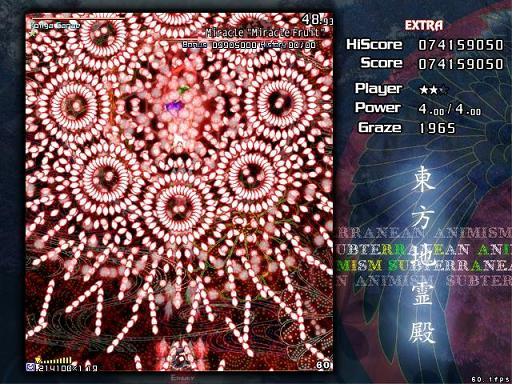
\includegraphics[scale=0.75]{fichiers_rapport/images/touhou_project.jpg}
\end{center}

L'objectif de notre projet est donc le suivant, créer un Manic Shooter. Il faut donc qu'il est les mêmes atouts et défauts que ce dernier. De ce fait, nous avons mis en place un place un moteur de jeu capable de gérer ce nombre immense de projectiles mais aussi d'ennemis.

Dans le cadre de ce jeu, nous avons crée un story-mode, une sorte de mode histoire ou des stages définis à l'avance s'enchainent et où les joueurs pourront tenter d'afficher le highscore. Ce mode se révèle très corsée contrairement au deuxième mode.

Ce deuxième mode en question est un mode où l'on génère de manière procédurale (c'est à dire que l'on imbrique aléatoirement plusieurs vagues d'ennemis prédéfinis) le niveau. Ainsi, en fonction de la difficulté, on obtient un niveau différent à chaque fois.

Suite à plusieurs problèmes, nous avons été obligé de ralentir la progression du jeu et n'avons ajouté des ennemis différents et la gestion du score que très tardivement. La génération de niveau et la majeure partie du moteur de jeu ont été fait pendant le premier semestre et la première moitié du deuxième semestre.

La deuxième moitié du deuxième semestre a été mise à profit pour équilibrer certains ennemis, modifier l'esthétique du jeu, créer de nouveaux ennemis ou encore gérer le highscore et le menu pause.

Nous allons désormais aborder le fonctionnement du jeu et ses mécaniques.

\section{Moteur du jeu}

\subsection{Le générateur de niveaux}

\section{Deuxième partie}



\section{Réalisation}



\section{Conclusion}



\end{document}
